% === Revised Section 7: What this buys us for LLMs ===

% NEW PREAMBLE ADDITIONS NEEDED:
% \usepackage{tikz}
% \usetikzlibrary{arrows.meta,positioning}
% \usepackage{listings}
% \lstset{basicstyle=\ttfamily\small,breaklines=true,frame=single,
%         backgroundcolor=\color{gray!5}}
% \newtcolorbox{activity}[1][]{
%   breakable, enhanced,
%   colback=blue!5, colframe=blue!60!black,
%   coltitle=white, fonttitle=\bfseries,
%   title={Activity}, boxrule=0.6pt,
%   left=6pt,right=6pt,top=4pt,bottom=4pt, #1}
% \newtcolorbox{story}[1][]{
%   breakable, enhanced,
%   colback=green!5, colframe=green!50!black,
%   coltitle=white, fonttitle=\bfseries,
%   title={A Short Story}, boxrule=0.6pt,
%   left=6pt,right=6pt,top=4pt,bottom=4pt, #1}

\section{What this buys us for LLMs}
\label{sec:llms}

\begin{intuition}
\textbf{The one-line version, for the coffee chat.}  A large language
model trained to guess the next word is, provably and mechanically,
a compressor of its training data.  That is not an analogy.  It is a
theorem (\cref{thm:ce-code}) plus a pipe (the arithmetic coder).
By the chain we built in \cref{eq:chain}, being a good compressor
puts the model somewhere on the intelligence spectrum defined by
Solomonoff (\cref{thm:solomonoff}).

\textbf{Residuals and arithmetic coding, in very plain English.}
At every token, the model publishes a probability for each possible
next word.  The \emph{residual} is the gap between that guess and
what actually happened.  If the model said "the" with probability
$0.9$ and "the" appeared, the residual is about $-\log_2 0.9 \approx
0.15$ bits --- almost free.  If the model said $0.01$ and "the" still
appeared, the residual is $-\log_2 0.01 \approx 6.6$ bits --- an
expensive surprise.  \emph{Arithmetic coding} is a near-optimal way
to write all those surprise numbers down back to back.  The
compressed file has two parts: the model weights (one fixed cost)
plus the bill for every surprise (variable cost).  Better model
$\Rightarrow$ fewer surprises $\Rightarrow$ smaller bill
$\Rightarrow$ shorter file.  "KL divergence", when we use it below,
is the same tax, averaged: the extra bits per token you pay for
betting on the wrong distribution.

\textbf{Three things a decision-maker should take away, up front.}
(1) Cross-entropy on your own domain data is a real yardstick ---
one number, comparable across vendors.  (2) "Just predict the next
word" is not marketing spin; the mathematics agrees that it produces
general-looking behaviour.  (3) There is a ceiling (the Shannon
entropy of the text).  As models approach it, cost per extra bit
goes vertical; the frontier moves to multimodal data, embodied
interaction, and reasoning architectures.  Plan capex accordingly.

\textbf{The Hutter Prize, concretely.}  Marcus Hutter put up a
$500{,}000$~\euro{} bounty for whoever compresses the first $1$~GB
of English Wikipedia (the \texttt{enwik9} file) the most
\citep{hutter2005universal}.  The current leaderboard is dominated
by neural compressors; as of early $2024$, Fabrice Bellard's
\texttt{nncp} sits near $0.113$ bits per character, down from
\texttt{gzip}'s $\sim 2.1$.  Training an LLM on Wikipedia to
minimise cross-entropy \emph{is} compressing Wikipedia; the model
weights plus arithmetic-coded residuals are the compressed file.
Better prediction $=$ smaller file $=$ (by \cref{thm:ce-code})
better distributional model $=$ (by \cref{thm:solomonoff}) closer
to the true generating process $=$ (per Hutter) more intelligence.

\textbf{Scaling laws.}  Plot model size against cross-entropy loss
on held-out text: you get a strikingly clean curve.  Double the
data, double the parameters, the loss drops predictably.  The curve
has been stable across four orders of magnitude
\citep{kaplan2020scaling}.  Cross-entropy --- our bits-per-token
yardstick --- is a smooth function of investment.  You can buy
intelligence by the bit: not efficiently, not forever, but
predictably.  \Cref{fig:scaling} sketches the shape.

\textbf{A worked example, in numbers.}  GPT-2 hit roughly $1.2$
bits per English character on the standard benchmark; GPT-4-class
models are around $0.7$.  That looks like a modest drop.  But
English text is about $1.3$ bits of true entropy per character
(Shannon's 1950s estimate).  So GPT-2 was at $\sim 92\%$ of the
way from "random guessing" ($\sim 5$ bpc) to the floor; GPT-4 is
at $\sim 98\%$.  Six percentage points.  Small in bits, enormous
in dollars: the last bit contains the reasoning, the rare facts,
the nuanced world-models.  \Cref{fig:lastmile} makes the cost
asymmetry visible.

\textbf{Emergent capabilities, cautious framing.}  If the training
objective is a compression proxy, and compression is provably
linked to a universal notion of intelligence, then an LLM doing
arithmetic, translation, and code --- capabilities nobody
explicitly trained for --- is consistent with the theory.  To
compress English well, you must model the world that the English
is about.  We resist the stronger claim that emergence is
\emph{predicted} by the theory; it is consistent, which is enough
for a capital-allocation argument.
\end{intuition}

\begin{story}
Two sales reps walk into your office on the same afternoon.  Rep~A
pitches a \emph{language model}: it writes emails, summarises
documents, drafts code.  KPI: user satisfaction.  Rep~B pitches a
\emph{Wikipedia compressor}: one number, bits-per-character, lower
is better.  You sign with Rep~A.  Three weeks later, legal calls:
Rep~A and Rep~B shipped the \emph{same binary}.  Different
marketing, same product.  That is the content of \cref{eq:chain}.
The KPI you choose to stare at determines which half of the
equivalence you buy, but the vendor was selling both all along.
\end{story}

\subsection*{The formal content}

A large language model parameterises a conditional distribution
$q_\theta(x_t \mid x_{<t})$ and is trained by minimising the
negative log-likelihood
\begin{equation}
  \mathcal{L}(\theta)
  \;=\; -\frac{1}{T}\sum_{t=1}^{T} \log_2 q_\theta(x_t \mid x_{<t}).
  \label{eq:llm-loss}
\end{equation}
By \cref{thm:ce-code}, $\mathcal{L}(\theta)$ is the expected
arithmetic-coding length per token: minimising cross-entropy
\emph{is} minimising compressed size.  Equivalently, by
\cref{cor:ppl}, a perplexity of $P$ corresponds to exactly
$\log_2 P$ bits per token --- e.g.\ perplexity $32$ is $5$~bits,
perplexity $8$ is $3$~bits.  A one-bit-per-token improvement on a
$100$~GB corpus saves, in principle, $\sim 12.5$~GB of code length.

\citet{kaplan2020scaling} showed that $\mathcal{L}(\theta)$ follows
clean power laws in model size $N$, dataset size $D$, and compute
$C$, of the form $\mathcal{L} \approx (N_c / N)^{\alpha_N}$.
Viewed through~\eqref{eq:llm-loss}, each such power-law decrement
is a \emph{bit-per-token compression improvement}.  The
operational content of \cref{thm:solomonoff} in this setting is
that, to the extent that the data-generating process is
computable, any predictor whose bits-per-token approaches the
conditional entropy rate $\overline{H}(p)$ (the theoretical
minimum achievable loss) is implicitly approximating the
$\mu$-posterior of the universal prior $M$.

\citet{deletang2024language} operationalised this equivalence by
wiring a large language model into an arithmetic coder and using
it to compress raw bytes of image and audio data.  They reported
compression ratios lower than domain-specific specialist
compressors (e.g.\ PNG, FLAC) on out-of-domain modalities, despite
the model having been trained solely on text.  From the vantage
point of \cref{thm:ce-code,thm:solomonoff}, the experiment is a
consistency check: a predictor that approximates a universal prior
should, by \eqref{eq:dominance}, compress any computable source to
within an additive $K(\mu)$ of its true entropy, and text exposure
turns out to be enough to learn a useful approximation of that
prior.

The \textbf{Hutter Prize} \citep{hutter2005universal} formalises
the economic version of the claim: a cash prize for improving the
lossless compression ratio on a fixed text corpus.  Within the
equivalence framework, every winning submission is, by definition,
a model whose cross-entropy on the corpus is lower --- which, by
\cref{cor:ppl}, is a more accurate next-symbol predictor.

\subsection*{Two pictures}

\begin{figure}[h]
\centering
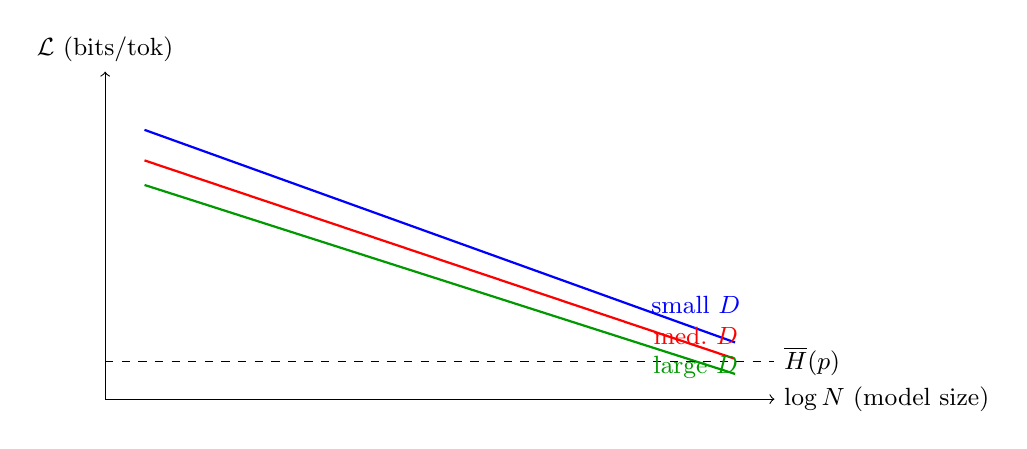
\begin{tikzpicture}[x=1cm,y=0.8cm]
  \draw[->] (0,0) -- (8.5,0) node[right] {\small $\log N$ (model size)};
  \draw[->] (0,0) -- (0,5.2) node[above] {\small $\mathcal{L}$ (bits/tok)};
  % three curves, different data sizes
  \draw[thick, blue]  plot[domain=0.5:8,samples=40] (\x, {4.5 - 0.45*\x});
  \draw[thick, red]   plot[domain=0.5:8,samples=40] (\x, {4.0 - 0.42*\x});
  \draw[thick, green!60!black] plot[domain=0.5:8,samples=40] (\x, {3.6 - 0.40*\x});
  \draw[dashed] (0,0.6) -- (8.5,0.6) node[right] {\small $\overline{H}(p)$};
  \node[blue] at (7.5,1.5) {\small small $D$};
  \node[red] at (7.5,1.0) {\small med.\ $D$};
  \node[green!60!black] at (7.5,0.5) {\small large $D$};
\end{tikzpicture}
\caption{Scaling laws \citep{kaplan2020scaling}.  Three curves, one
per dataset size; all three asymptote to the conditional entropy
floor $\overline{H}(p)$ (dashed).  Doubling $N$ gives a predictable
$\alpha_N$-sized drop in bits per token.}
\label{fig:scaling}
\end{figure}

\begin{figure}[h]
\centering
\begin{tikzpicture}[x=1.2cm,y=0.9cm]
  \draw[->] (0,0) -- (7.5,0) node[right] {\small \% of way to $\overline{H}(p)$};
  \draw[->] (0,0) -- (0,5.2) node[above] {\small $\log(\$ \text{ per bit})$};
  \draw[thick, red] plot[domain=0.2:6.9,samples=60]
        (\x, {0.3 + 0.15*\x + 0.25*exp(0.9*(\x-5))});
  \node at (1.5,-0.4) {\small $50\%$};
  \node at (3.5,-0.4) {\small $80\%$};
  \node at (5.0,-0.4) {\small $92\%$ (GPT-2)};
  \node at (6.5,-0.4) {\small $98\%$ (GPT-4)};
  \draw[dashed] (5.0,0) -- (5.0,1.5);
  \draw[dashed] (6.5,0) -- (6.5,4.5);
\end{tikzpicture}
\caption{The last-mile argument.  Cost per additional bit below the
Shannon floor climbs exponentially.  Moving from GPT-2's $92\%$ to
GPT-4's $98\%$ is six percentage points on the x-axis and several
orders of magnitude on the y-axis.  The curve is schematic; the
shape is what matters.}
\label{fig:lastmile}
\end{figure}

\subsection*{The working equivalence}

Collecting the theorems of \crefrange{sec:pred-comp}{sec:aixi} we
obtain the \emph{working equivalence}, first in English, then in
symbols.

\medskip
\noindent\textbf{In English.}  \emph{A model that predicts text
well is, by theorem, a model that compresses text well, and a model
that compresses text well is, by theorem, an approximation of the
universal prior that defines Solomonoff's notion of intelligence.}
One object, three KPIs.

\medskip
\noindent\textbf{In symbols:}
\begin{equation}
  \underbrace{\text{low cross-entropy}}_{\text{good predictor}}
  \;\Longleftrightarrow\;
  \underbrace{\text{short arithmetic code}}_{\text{good compressor}}
  \;\Longleftrightarrow\;
  \underbrace{\text{approx.\ of universal prior}}_{\substack{\text{Solomonoff/AIXI}\\\text{sense of intelligence}}}
  \label{eq:chain}
\end{equation}
The leftmost arrow is a theorem within Shannon's framework
(\cref{thm:ce-code}).  The rightmost arrow is an asymptotic
theorem modulo computability (\cref{thm:solomonoff}).  Neither is
a metaphor.

\subsection*{Activities}

\begin{activity}[title={Activity 1 --- Hutter Prize bingo}]
Project the current Hutter Prize leaderboard
(\url{http://prize.hutter1.net}).  Each student writes down, on a
sticky note, who they think wins the $2030$ title: (a) a
transformer LLM plugged into \texttt{nncp}-style arithmetic coder;
(b) a state-space model (Mamba-like); (c) a diffusion-based token
model; (d) a symbolic/hybrid system; (e) "none --- the leaderboard
plateaus at $\sim 0.10$ bpc".  Collect notes, tally, revisit at the
end of term.  \emph{Helps Yuki} (concrete artefact),
\emph{helps Maria} (named numbers).
\end{activity}

\begin{activity}[title={Activity 2 --- LLM as compressor (Python)}]
Run this snippet locally.  It wires \texttt{gpt2-small} into a
simple arithmetic coder and compresses a $10$~KB sample of
\texttt{enwik8}.  Report bytes in, bytes out, and the ratio
against \texttt{gzip}.
\begin{lstlisting}[language=Python]
import gzip, math, torch
from transformers import GPT2LMHeadModel, GPT2TokenizerFast
# Load model + tokenizer
tok = GPT2TokenizerFast.from_pretrained("gpt2")
mdl = GPT2LMHeadModel.from_pretrained("gpt2").eval()
# Load 10 KB of enwik8
with open("enwik8_10kb.txt") as f: text = f.read()
ids = tok.encode(text, return_tensors="pt")
# Compute summed negative log-likelihood -> bits
with torch.no_grad():
    logits = mdl(ids).logits[:, :-1, :]
    logp   = torch.log_softmax(logits, dim=-1)
    targets = ids[:, 1:]
    nll = -logp.gather(2, targets.unsqueeze(-1)).sum().item()
bits_gpt2 = nll / math.log(2)
bytes_gzip = len(gzip.compress(text.encode()))
print(f"raw        : {len(text):>7d} bytes")
print(f"gzip       : {bytes_gzip:>7d} bytes")
print(f"gpt2 code  : {bits_gpt2/8:>7.0f} bytes  (+model weights)")
\end{lstlisting}
Discussion: where does the model-weights cost go?  At what corpus
size does the weights amortise?  \emph{Helps Leo} (hands-on),
\emph{answers Maria's falsifiability demand}.
\end{activity}

\begin{activity}[title={Activity 3 --- Perplexity-to-bits worksheet}]
Fill in the table.  Assume $100$~GB of English text.
\medskip

\noindent
\begin{tabular}{lccc}
\hline
Model           & Perplexity & Bits/token & Storage (GB) \\
\hline
n-gram baseline & $128$      & \rule{1.5cm}{0.3pt} & \rule{1.5cm}{0.3pt} \\
GPT-2           & $32$       & \rule{1.5cm}{0.3pt} & \rule{1.5cm}{0.3pt} \\
GPT-4 class     & $8$        & \rule{1.5cm}{0.3pt} & \rule{1.5cm}{0.3pt} \\
Shannon floor   & $\approx 5.3$ & \rule{1.5cm}{0.3pt} & \rule{1.5cm}{0.3pt} \\
\hline
\end{tabular}

\medskip
Hint: bits/token $= \log_2(\text{perplexity})$.  Assume $4$
characters per token; $1$ byte per character in raw text.
Answers: $7, 5, 3, 2.4$ bits/tok.  \emph{Helps Leo}
(do-able on paper), \emph{helps Aisha} (she can now say the
sentence "perplexity $32$ means $5$ bits per token").
\end{activity}

\begin{activity}[title={Activity 4 --- Two-vendors role-play}]
Two students play Rep~A (sells "a language model") and Rep~B
(sells "a Wikipedia compressor").  Each has two minutes and one
KPI.  The class, acting as buyer, asks questions.  Debrief
question: "If the binary is the same, which KPI should your CFO
actually track?"  Answer keys: cross-entropy on in-domain eval
data; it happens to be both KPIs at once.  \emph{Helps Yuki}
(picture), \emph{helps Aisha} (language for the board).
\end{activity}

% =========================================================================
